\section{Урвуу инженерчлэл: "Auftragsverwaltung" систем дэх зохиомжийн үлгэр загварууд}
Энэ хэсэгт Жава технологийг ашиглан хэрэгжүүлсэн бараа захиалгийг зохицуулах Герман нэршлийн конвенцтэй "Auftragsverwaltung" систем дээр урвуу инженерчлэлийн аргачлалаар програм хангамжийн зохиомжийн үлгэр загваруудыг уг системд хэрхэн ашигласан байгааг олж тогтооно.

\subsection{Системийн статик загвар}
Системийн классын диаграмыг гаргахын тулд Eclipse IDE дээрх PlantUML\footnote{https://plantuml.com/eclipse} програм хангамжийн багажыг ашигласан. Гэвч энэ багаж нь классууд хоорондын холбоосуудыг, тухайлбал бүрдмэл, нийлмэл зэрэг холбоог оновчтой гаргаж чадаагүй. Юуны түрүүнд энэ системийн нэршлийн конвенц нь Герман хэл дээр хийгдсэн учир тодорхой үгсийн Герман–Англи нэршлийн конвенцийг гаргах шаардлага үүссэн. Жишээ нь, "Auftragsverwaltung" нь "OrderManagement" буюу захиалгын удирдлага, "Auftrag" нь Order" буюу захиалга, "Kunde" нь "Customer" буюу харилцагч, "auftragLoeschen" нь "deleteOrder" буюу Order (Aufrag) классын устгагч гэх мэт. Хавсралт B хэсгээс эдгээр орчуулгыг харж болно.

Холбоосуудын төрлийг тодорхойлохын тулд класс тус бүрийн устгагчийн хэрэгжүүлэлтийг ажигласан. Жишээ нь, Order (Aufrag), OrderItem (Aufragsposition) классуудын хувьд Order классын объектийг устгах үед OrderItem классын объектуудаас бүрдсэн вектороор entfernenPos аргын тусламжтай гүйж устгаж байна. Харин Customer (Kunde) классын объектыг устгалгүй үлдээсэн байна. Иймд Order, OrderItem классууд хоорондоо нийлмэл холбоотой бол Order, Customer классууд хоорондоо бүрдмэл холбоотой гэж дүгнэлээ.
\begin{lstlisting}[language=Java, caption=Order классын устгагч auftragLoeschen, frame=single]
public boolean entfernenPos(Auftragsposition apos)
{
    boolean rc = apositionen.remove(apos);
    if (rc)
        this.aktualisieren();
    return rc;
}

public void auftragLoeschen()
{
    Iterator<Auftragsposition> positionen =
            apositionen.iterator();
    while (positionen.hasNext())
    {
        entfernenPos(positionen.next());
    }
}
\end{lstlisting}

Үүнтэй адилаар "Applicationlogic" багцын бүх классын нэрсийг жагсааж, тэдгээрийн хоорон -дын холбоосуудыг илрүүлсэн. Дараа нь, холбоосуудын төрлийг тодорхойлж, UML классын диаграмыг гаргасан. Үүний үр дүнг \ref{fig:diagram1} зурагт үзүүлэв. Мөн Item (Artikel) класс нь гадаад "Utility" багцаас (зураг \ref{fig:diagram4})\quad Money (Geld) классыг ашиглаж байгаа тул энэ холбоосыг харуу -лаагүй болно.

\begin{figure}
	\centering
	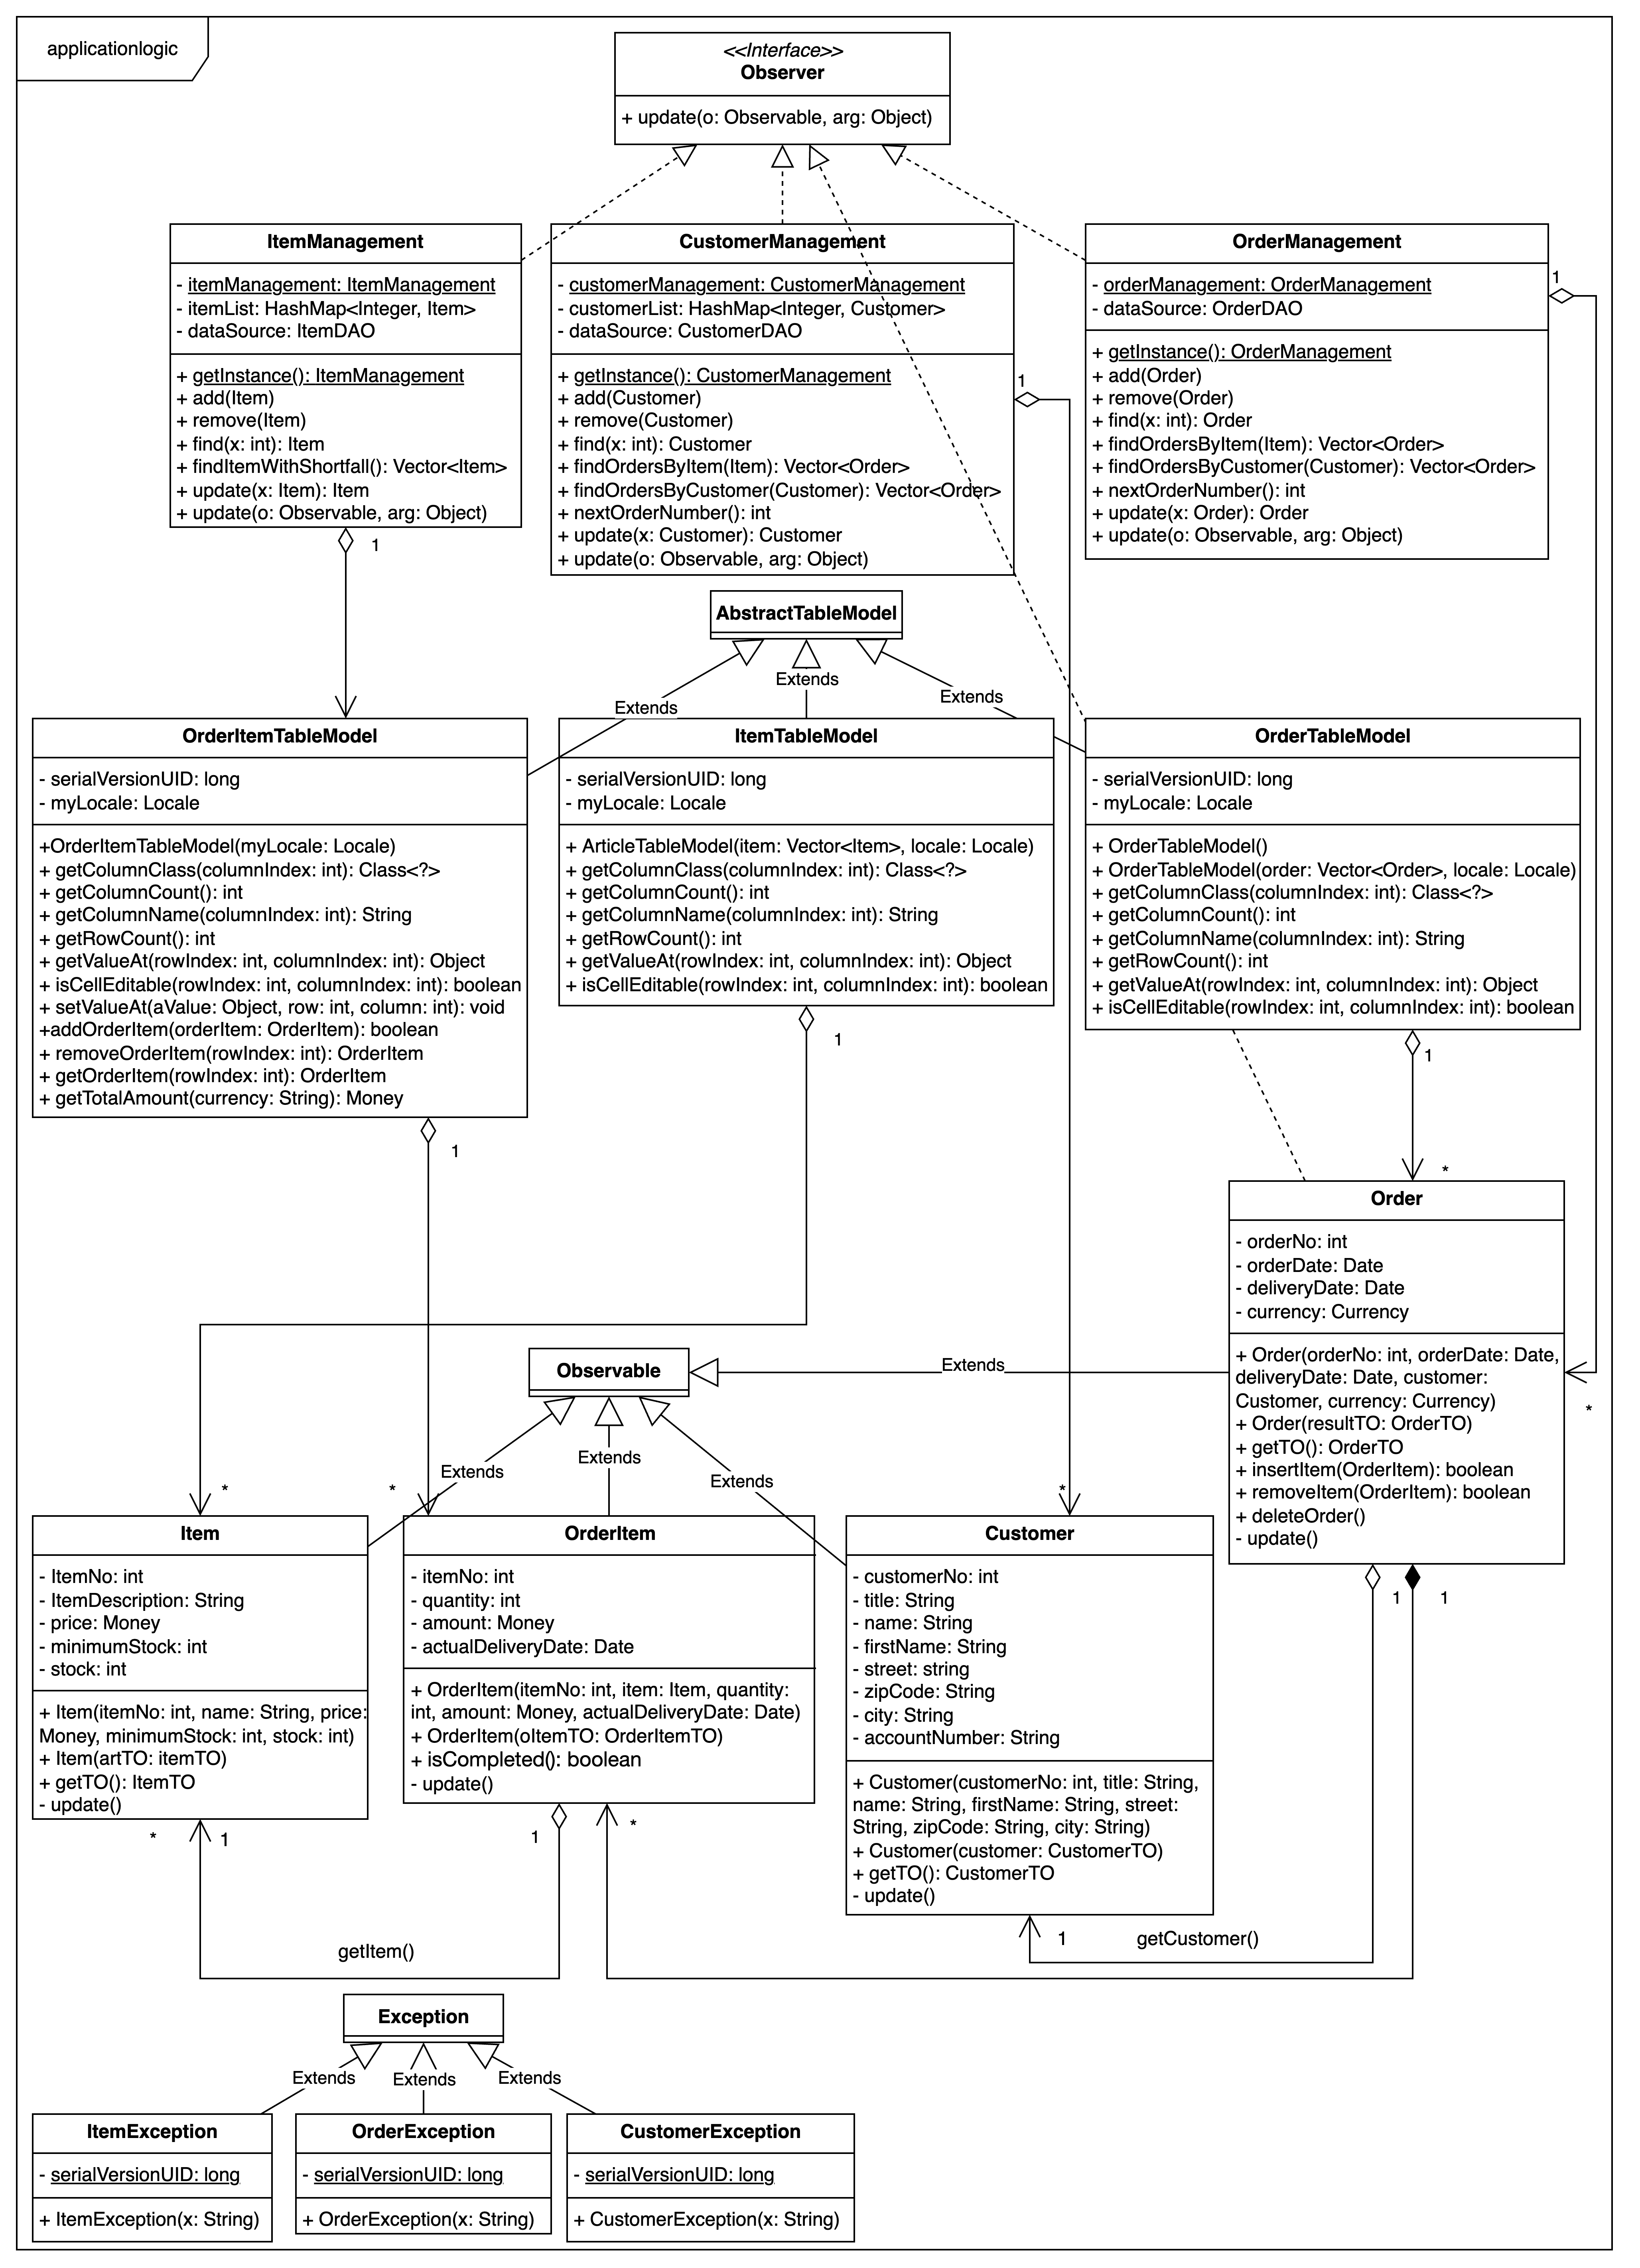
\includegraphics[width=15cm]{images/diagram1.png}
	\caption{"Applicationlogic" багцын классын диаграм}
	\label{fig:diagram1}
\end{figure}

\begin{figure}
	\centering
	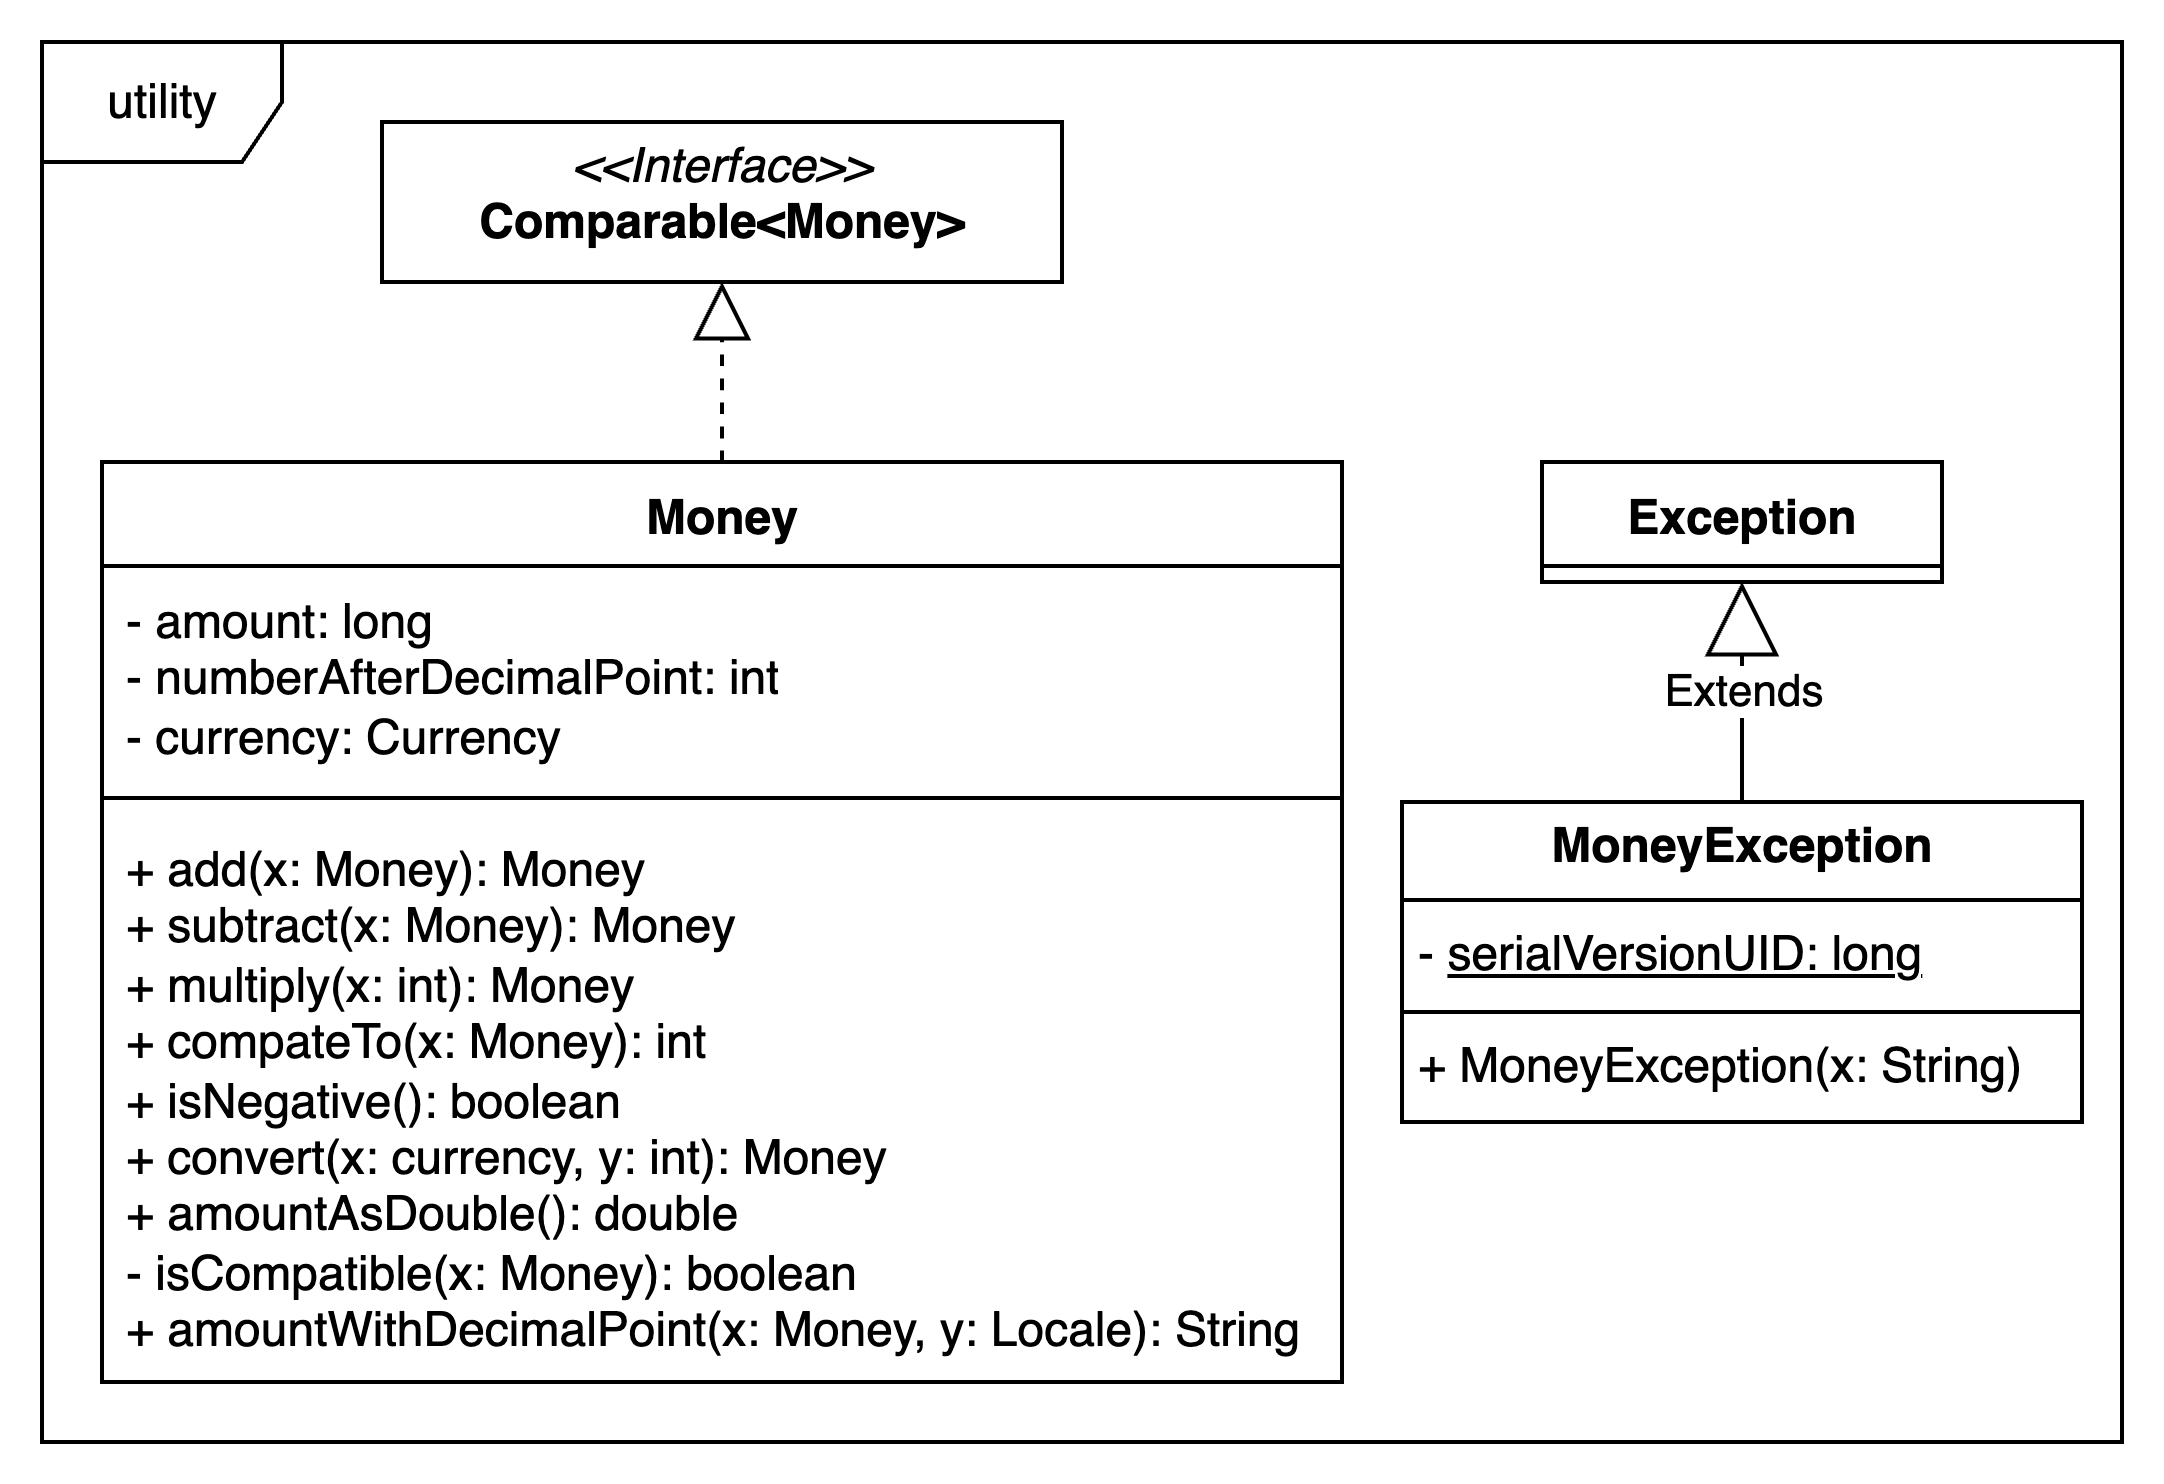
\includegraphics[width=10cm]{images/diagram4.png}
	\caption{"Utility" багцын классын диаграм}
	\label{fig:diagram4}
\end{figure}

\subsection{Системийн зохиомж}
Энэ хэсэгт "Auftragsverwaltung" системд илрүүлсэн гол зохиомжийн үлгэр загваруудын зорилго, хэрэглээ, бүтцийн элемент, өмнө тулгарч болох асуудал, үр дүн, жишээ код болон систем доторх бодит хэрэгжүүлэлтийг дэлгэрэнгүй авч үзнэ.

\subsubsection{"Iterator" үлгэр загвар}
Order классын бүх талбар, аргуудаар статик уншлага хийн \verb|apositionen.iterator()|,\\ \verb|while (positionen.hasNext())|,\verb| positionen.next()| мөрүүдийг тэмдэглэж үлгэр загварт заавал байх элементүүд кодод ямар хэлбэрээр илэрсэнг харлаа. Энд apositionen нь \textit{бүрдэл} болж, түүний \verb|iterator()| аргыг дуудаж байгаа нь "Iterator" интерфэйсийг ашиглаж буйг илтгэнэ. \verb|auftragLoeschen()| болон \verb|getAuftragssumme()| мэт аргуудын давталтын логикыг уншиж, хэрхэн давталт явдаг, давталтын үед ямар үйлдэл хийгдэхийг тодруулсан. Давталтын туршид бүрдлүүдтэй хэрхэн харьцаж байгааг анхааран харж, "concurrent modification"\footnote{Конкуррент програмчлалд өгөгдлийн бүтцийг өөр процесс эсвэл тредээр давтаж байх үед өөрчилсөн тохиолдолд "concurrent modification" үүсдэг. Энэ нь үнэн байхаа больсон өгөгдлийн бүтцээр гүйснээс үүдсэн урьдчилан таамаглах боломжгүй өгөгдлийн эвдрэл эсвэл "runtime error" алдааг үүсгэж болно.} зэрэг асуудал үүсэх эрсдлийг тооцсон. Дээрх ажиглалтаас үлгэр загварын шинж тэмдгүүд илэрсэн тул тухайн кодонд "Iterator" үлгэр загвар ашиглагдсан гэж тодорхойлсон. Энд apositionen нь \verb|Vector<Auftragsposition>| бөгөөд давталт хийхдээ \verb|apositionen.iterator()| ашиглагдаж байна. \verb|getAuftragssumme()| нь \verb|while(positionen.hasNext()){...positionen.next()...}| маягаар стандарт давталтыг ашиглан бүх Amount (Betrag) буюу үнийн дүнг олж байна. Энэ нь "Iterator" интерфэйсийн классик хэрэглээ юм.

\begin{lstlisting}[language=Java, caption=Order классын арга getAuftragssumme, frame=single]
  public Geld getAuftragssumme()
  {
    Iterator<Auftragsposition> positionen =
        apositionen.iterator();
    Geld ergebnis = new Geld(0, 0, waehrung);
    if (positionen.hasNext())
      ergebnis = new Geld(positionen.next().getBetrag());
    while (positionen.hasNext())
    {
      ergebnis.addieren(positionen.next().getBetrag());
    }
    return ergebnis;
  }
\end{lstlisting}

\subsubsection{"Singleton" үлгэр загвар}
OrderManagement классын статик талбар дээр шууд \verb|new Auftragsverwaltung()| дуудаж байгаа нь "eager initialization"\footnote{"Eager initialization" нь програмчлалын стратеги бөгөөд объект эсвэл нөөцийг анх ашиглахыг хүсэх хүртэл хүлээх биш, агуулагдсан класс нь ачаалагдсан даруйд үүсгэгддэг.} бөгөөд тредүүдэд аюулгүй байдаг боловч хэзээ ч ашиглагдахгүй объект байгуулагдах эрсдэлтэй. Мөн \verb|DAOFactory.getInstance()| гэх мэт глобал хандалтын цэгүүдийг ажиглалаа.   Класс нь өөрөө "Observer"-ыг хэрэгжүүлж, менежментийн үүрэг гүйцэт- гэж байгаа ч байгуулагчийг private гэж огт заагаагүй тул шинэ Auftragsverwaltung объектыг байгуулж параллел объект үүсгэх эрсдэлтэй. \verb|hinzufuegen()| дотор \verb|auf.addObserver(this)| гэж байгаа нь Singleton объект өөрөө Observable объектын өөрчлөлтийг хүлээн авч DAO-руу өөрчлөлт илгээж байна. Энэ бүх ажиглалтуудаас жинхэнэ "Singleton" үлгэр загварыг ашиглаагүй гэж дүгнэлээ. Харин өөр нэг үлгэр загварыг олсон нь "Observer" юм. Үүнийг дараагийн хэсэгт тайлбарлав.
\begin{lstlisting}[language=Java, caption=OrderManagement классын арга hinzufuegen, frame=single]
  private static Auftragsverwaltung eineAuftragsverwaltung = new Auftragsverwaltung();

  public void hinzufuegen(Auftrag auf)
      throws AuftragException
  {
    int auftragsnr = auf.getAuftragsnr();
    try {
      if (datenquelle.read(auftragsnr) != null)
        throw new AuftragException(
            "Auftrag mit dieser Nummer ist schon vorhanden");
      datenquelle.create(auf.getTO());
      auf.addObserver(this);
    } catch (Exception ex)
    {
      throw new AuftragException("Auftrag " + auftragsnr
          + " konnte nicht gespeichert werden!");
    }
  }
\end{lstlisting}

\subsubsection{"Observer" үлгэр загвар}

OrderManagement классын \verb|hinzufuegen()| арга дотор \verb|auf.addObserver(this)| гэж байгаа нь Singleton объект өөрөө Observable объектын өөрчлөлтийг хүлээн авч DAO\footnote{"Data Access Object" нь өгөгдлийн нөөцтэй холбоотой бүх үйлдлийг багтааж, хийсвэрлэдэг тусгай давхаргын үүрэг гүйцэтгэдэг ба програмын үлдсэн хэсэг нь өгөгдөл хэрхэн, хаана хадгалагдаж байгаагаас хамааралгүй байх боломжийг олгодог.}-руу өөрчлөлт илгээж байна. Үүнийг ажигласнаар "Observer" үлгэр загвар ашиглагдсан гэж дүгнэлээ. Домайн объект болох Customer, Order, OrderItem, Item зэрэг классууд нь Observable-ээс удамшиж, өөрийн төлөв өөрчлөгдөх мөчид \verb|notifyObservers()|-ыг дуудаж бүх бүртгэлтэй Observer-уудад мэдээлж байна. CustomerManagement, OrderManagement, ItemManagement зэрэг класс нь Observer интерфейсийг хэрэгжүүлэн, \verb|update()| аргаар домайн объектоос ирсэн өөрчлөлтийг хүлээн авч байна. Ингэснээр системийн бүх чухал домэйн объектууд үзэгдлийн төв болж, менежер бүр эдгээр үзэгдлийг сонсож, өөрийн цуглуулгад харгалзах домэйн объектыг дахин оруулах/шинэчлэх нь төвлөрсөн удирдлага үүсгэхээс гадна домэйн объект, менежерүү- дийн хооронд нягт уялдаа холбоог бий болгож, нийцэмжтэй байдлыг хадгалж байна.

\subsubsection{"Composite" үлгэр загвар}
\verb|DAO<T extensions TransferObject>| интерфэйсийг хэрэгжүүлж болон стандарт CRUD үйлд- лүүд (create, read, update, delete) дээр нэмээд \verb|nextKey()|-ийг зарлаж, \verb|Iterable<T>|-г хүртэл өргөтгөсөн байна.
\begin{figure}
	\centering
	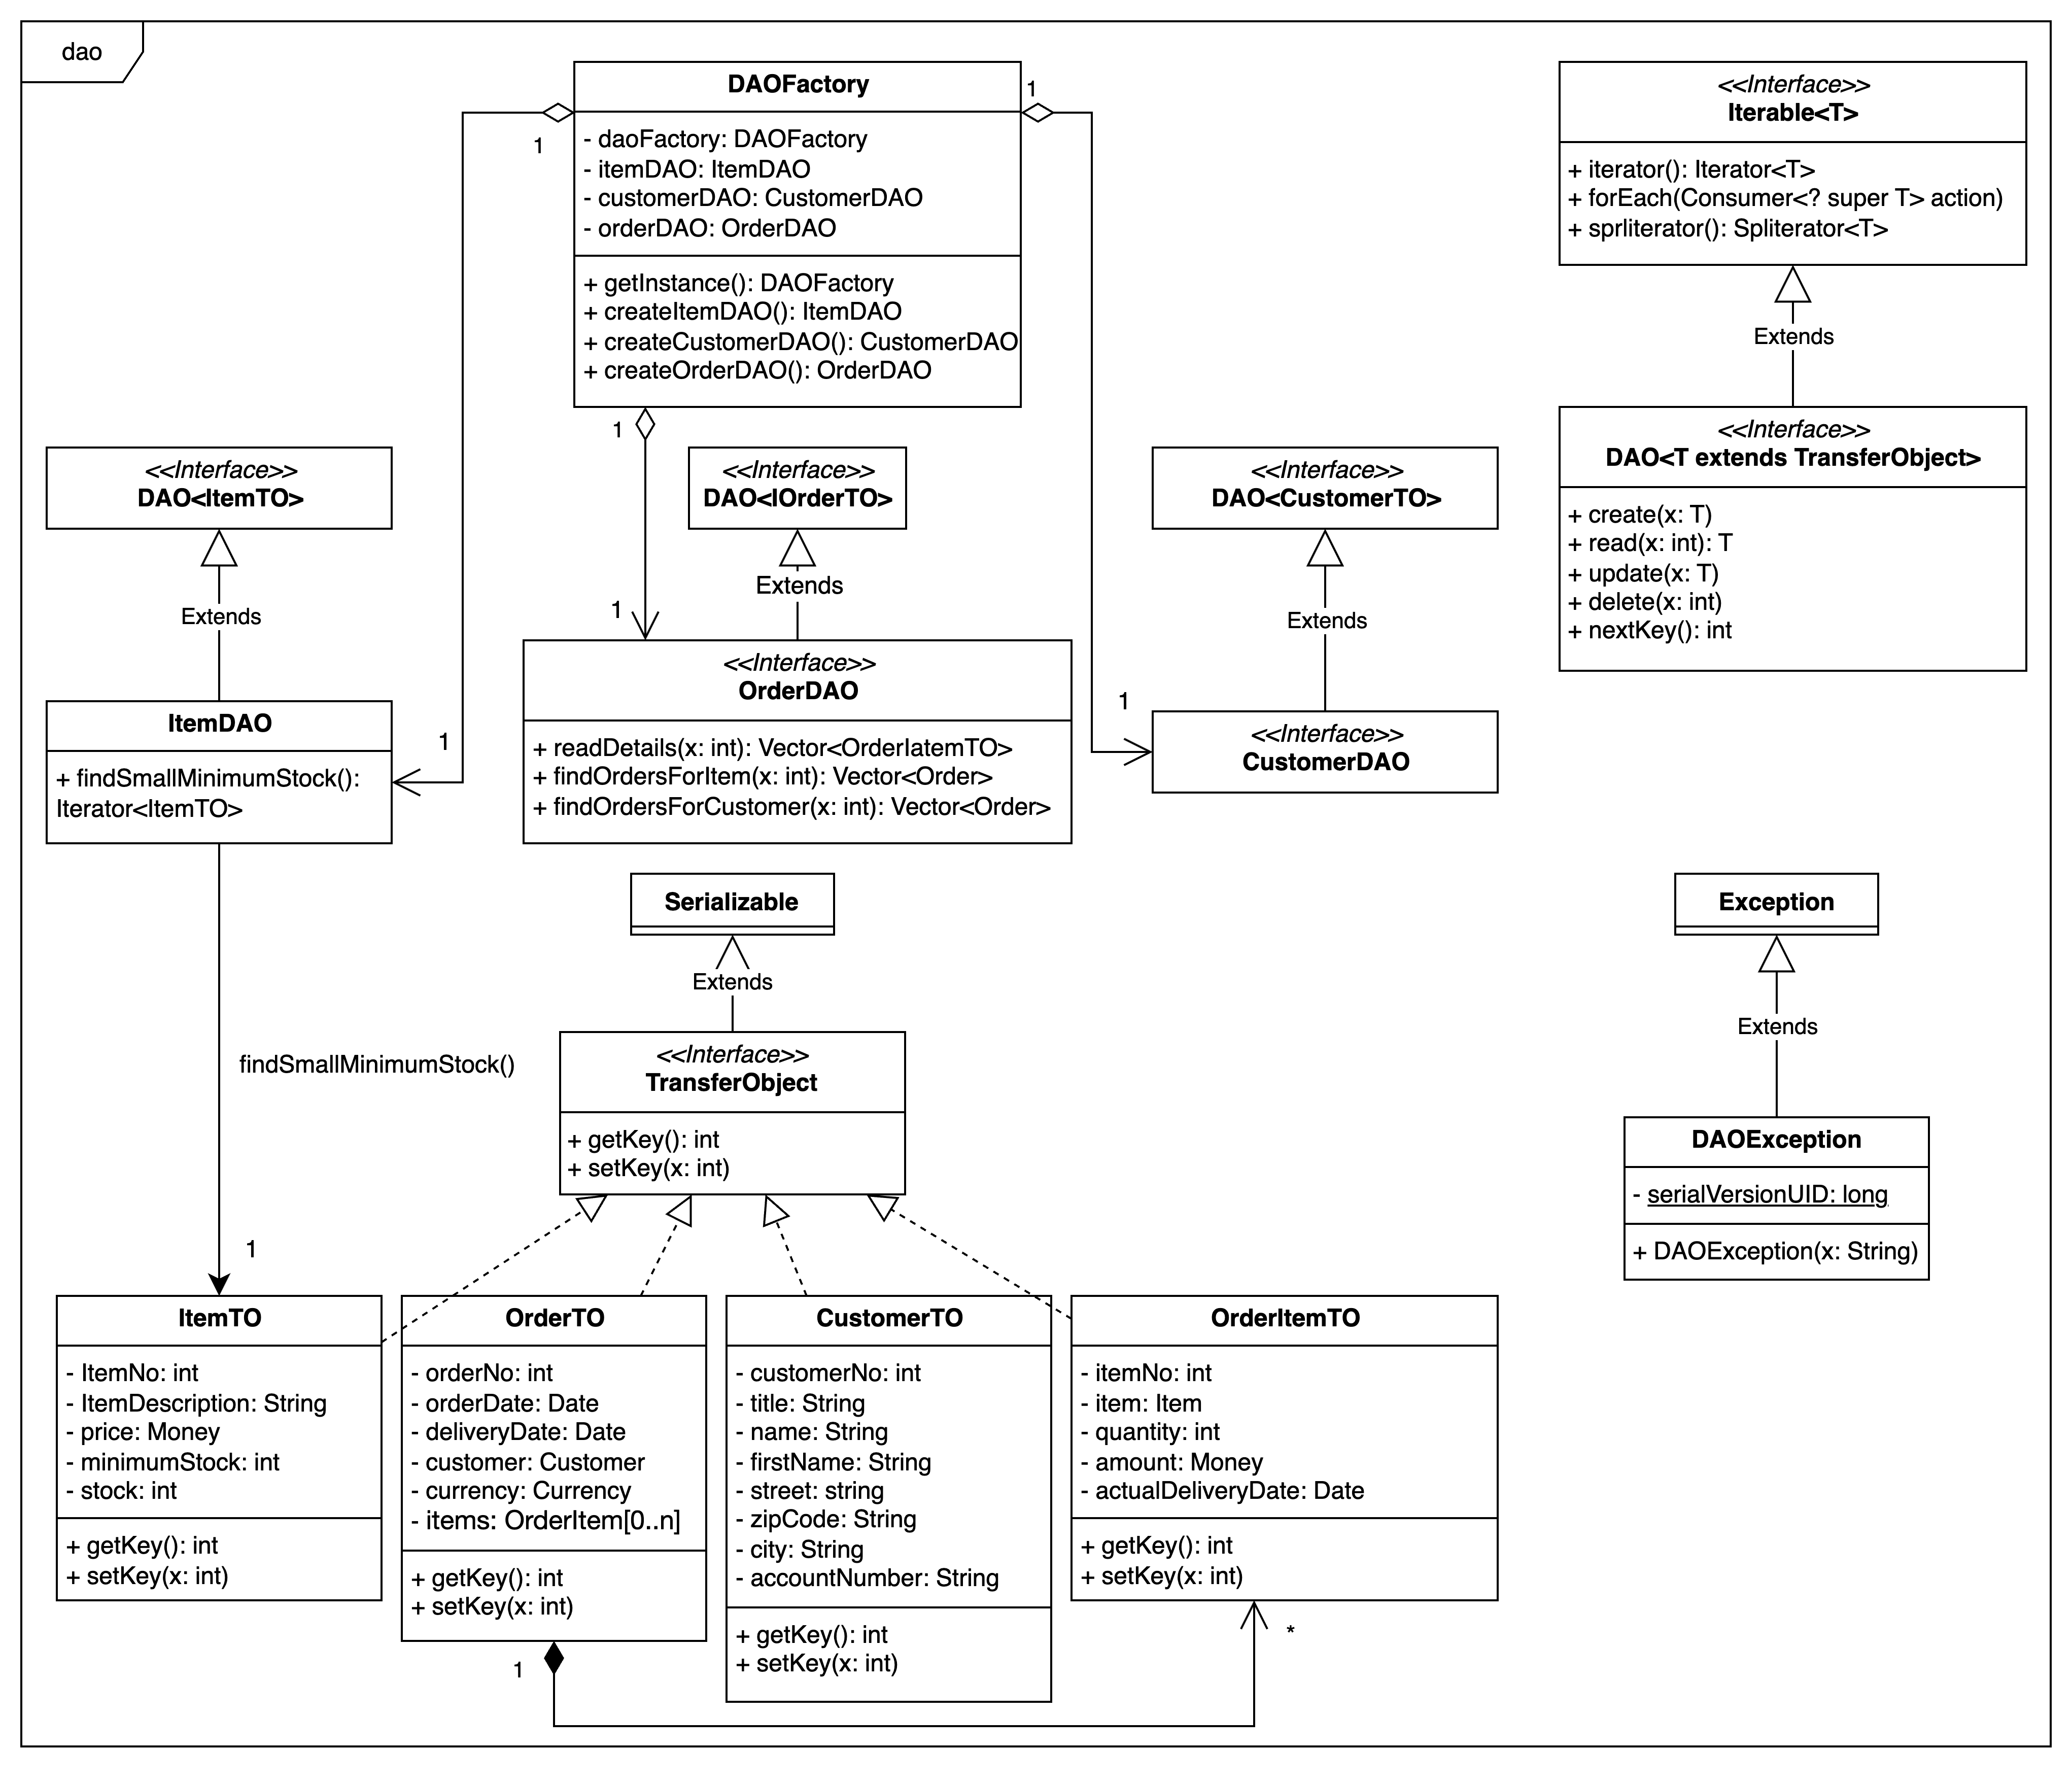
\includegraphics[width=15cm]{images/diagram3.png}
	\caption{"DAO" багцын классын диаграм}
	\label{fig:diagram3}
\end{figure}
Энэ нь DAO интерфэйсийг хэрэгжүүлсэн класс бүр нь өөрийн төрөлд харгалзах домэйн объектын цуглуулгыг удирдах үүрэгтэй болохыг илтгэнэ. Жишээ нь, доорх кодонд CustomerDAO нь Customer домэйн объектын цуглуулгыг удирдаж байна. Үүнийг ажигласнаар "Composite" үлгэр загвар ашиглагдсан гэж дүгнэлээ. Учир нь DAO интерфэйсийг хэрэгжүүлсэн класс бүр нь өөрийн төрөлд харгалзах домэйн объектын цуглуулгыг удирдах үүрэгтэй бөгөөд эдгээр DAO-уудын цуглуулга нь системийн бүх домэйн объектын цуглуулгыг бүрдүүлж байна. Энэ нь "Composite" үлгэр загварын үндсэн шинж чанар юм.\\

\begin{lstlisting}[language=Java, caption=KundeTO класс, frame=single]
public class KundeTO implements TransferObject
{
	...
  public KundeTO(int kundennr, String anrede, String name,
      String vorname, String ort, String plz,
      String strasse, String debitorennr)
  {
    this.kundennr = kundennr;
    this.anrede = anrede;
    this.name = name;
    this.vorname = vorname;
    this.strasse = strasse;
    this.plz = plz;
    this.ort = ort;
    this.debitorennr = debitorennr;
  }

  public int getKey()
  {
    return kundennr;
  }
  public void setKey(int newKey)
  {
    kundennr = newKey;
  }
}
\end{lstlisting}

\subsection{Дэд хэсгийн дүгнэлт}
Энэ хэсэгт “Auftragsverwaltung” системийг урвуу инженерчлэлийн аргаар задлан шинжилж, статик загвар, нэршлийн конвенци, мөн систем дотор илэрсэн гол зохиомжийн үлгэр загваруу- дыг тодрууллаа. Ерөнхий ажиглалт нь дараах үндсэн үр дүнг илэрхийлж байна:

\begin{itemize}
\item \textbf{Илрүүлсэн үлгэр загварууд:}
\begin{itemize}
\item \emph{Iterator:} \verb|apositionen.iterator()| болон стандарт давталтын логик ашиглагдсан нь Iterator үлгэр загварын тод илрэл юм; мөн давталтын явцад concurrent modification эрсдэл бий болж магадгүйг ажигласан.
\item \emph{Observer:} Домайн объектууд Observable-ээс удамшиж, менежер класс Observer-ийг хэрэгжүүлэн \verb|update()| аргыг ашиглаж байсан гэдгээс Observer загвар бодитоор ашиглагдсан.
\item \emph{Singleton (төстэй):} Auftragsverwaltung-д eager initialization хэлбэрийн статик талбар байгаа боловч private байгуулагчгүй тул жинхэнэ Singleton гэж дүгнэхэд хүрэлцэхгүй; мөн \verb|DAOFactory.getInstance()| гэх мэт глобал хандалтын цэгүүд ажиглагдсан.
\item \emph{Composite:} \verb|DAO<T extends TransferObject>|интерфэйс нь өөрийн төрөлд харгал- зах домайн объектын цуглуулгыг удирдаж байсан, энэ нь composite шинжтэй архи- тектурын хэрэглээ гэж тодорхойлсон.
\end{itemize}
\item \textbf{Системийн сайжруулалтын зөвлөмжүүд (ажил хэрэгжүүлэхэд туслах):}
\begin{itemize}
\item Iterator-д объект устгах үед \verb|Iterator.remove()| эсвэл Copy-on-write\footnote{"Copy-on-write" (CoW) нь өгөгдлийг өөрчлөх хүртэл хуулбарлахыг хойшлуулдаг оновчлолын стратеги юм.} ашиглах замаар concurrent modification-ыг арилгах
\item Singleton үлгэр загвар шаардлагатай бол private байгуулагч болон статик хандагч эсвэл enum-singleton ашиглан жинхэнэ Singleton-г баталгаажуулах; эсвэл глобал статик хандалтыг хязгаарлахын тулд dependency injection ашиглах.
\end{itemize}
\end{itemize}

Ерөнхийд нь, урвуу инженерчлэлийн үр дүнд “Auftragsverwaltung” систем нь хэд хэдэн түгээмэл зохиомжийн үлгэр загварыг бодитоор ашигласан болох нь нотлогдов. Гэхдээ зарим хэрэгжүүлэлт нь бүрэн биш ба конкуррент, глобал хандалтын менежмент зэрэг талуудыг сайжруулснаар системийн нийцтэй байдал, засвар үйлчилгээ илт сайжрах боломжтой. Энэ дүгнэлтийг үндэслэн дараагийн алхмууд нь кодын цэгцлэлт, synchronization/collection хяналт болон архитектурын жижиг рефакторууд байх ёстой гэж үзлээ.

\section{МУИС-ийн дипломын ажлыг удирдах системийн зохиомж дахь үлгэр загваруудын хэрэглээ}
Энэ хэсэгт МУИС-ийн дипломын ажлыг удирдах системийн зохиомжийг дадлага удирдагч Х. Ганзоригийн судалгааны ажилд тусгасан шаардлагын дагуу  зохиомжийн үлгэр загварууд, зохиомжийн зарчмуудыг ашиглан гаргасан.
\begin{itemize}
	\item \textbf{Singleton:} DepartmentManager, PlagiarismChecker зэрэг глобал менежерүүдийг нэг экземп- лярт хязгаарлах зорилгоор private constructor, static хандагчтай "singleton" үлгэр загварыг ашигласан.
	\item \textbf{Observer:} MilestoneTracker, Student, Supervisor, DepartmentHead зэрэг оролцогчид явцын мэдээлэл, дипломын ажлын статус өөрчлөгдөхөд update мэдэгдэл авах "observer pattern" үлгэр загварыг ашигласан. Жишээ нь, MilestoneTracker нь дипломын ажилд бүртгэгдэж, явцын өөрчлөлт бүрт метрик тооцоолон тайлан гаргадаг байна.
	\item \textbf{Composite:} Department, Committee, StudentGroup зэрэг цуглуулга объектыг бүрдмэл бүтэцтэйгээр удирдах зорилгоор "composite" үлгэр загварыг ашигласан. Жишээ нь, Committee нь гишүүдээс бүрдэж, үнэлгээ нэгтгэх, хамгаалалт зохион байгуулах үйлдлийг цогцоор нь гүйцэтгэдэг.
	\item \textbf{Factory:} ReportGeneratorFactory, EvaluatorFactory зэрэг нь тайлан, үнэлгээний генератор объектыг төрөл бүрээр үүсгэхэд "factory" үлгэр загварыг ашигласан.
	\item \textbf{Enum, Interface, Abstract class:} Статус, тайлангийн төрөл, milestone зэрэг enum-ууд, IEvaluator, IReportGenerator зэрэг интерфейс, Report зэрэг хийсвэр классуудыг ашиглан системийн өргөтгөх боломж, стандартчиллыг хангаж өгсөн.
\end{itemize}

Холбоосуудыг UML стандартын дагуу (aggregation, composition, dependency, realization) тэмдэглэсэн. Гэвч одоогоор үлгэр загваруудыг бодит кодын түвшинд хэрэгжүүлээгүй.
\begin{figure}
	\centering
	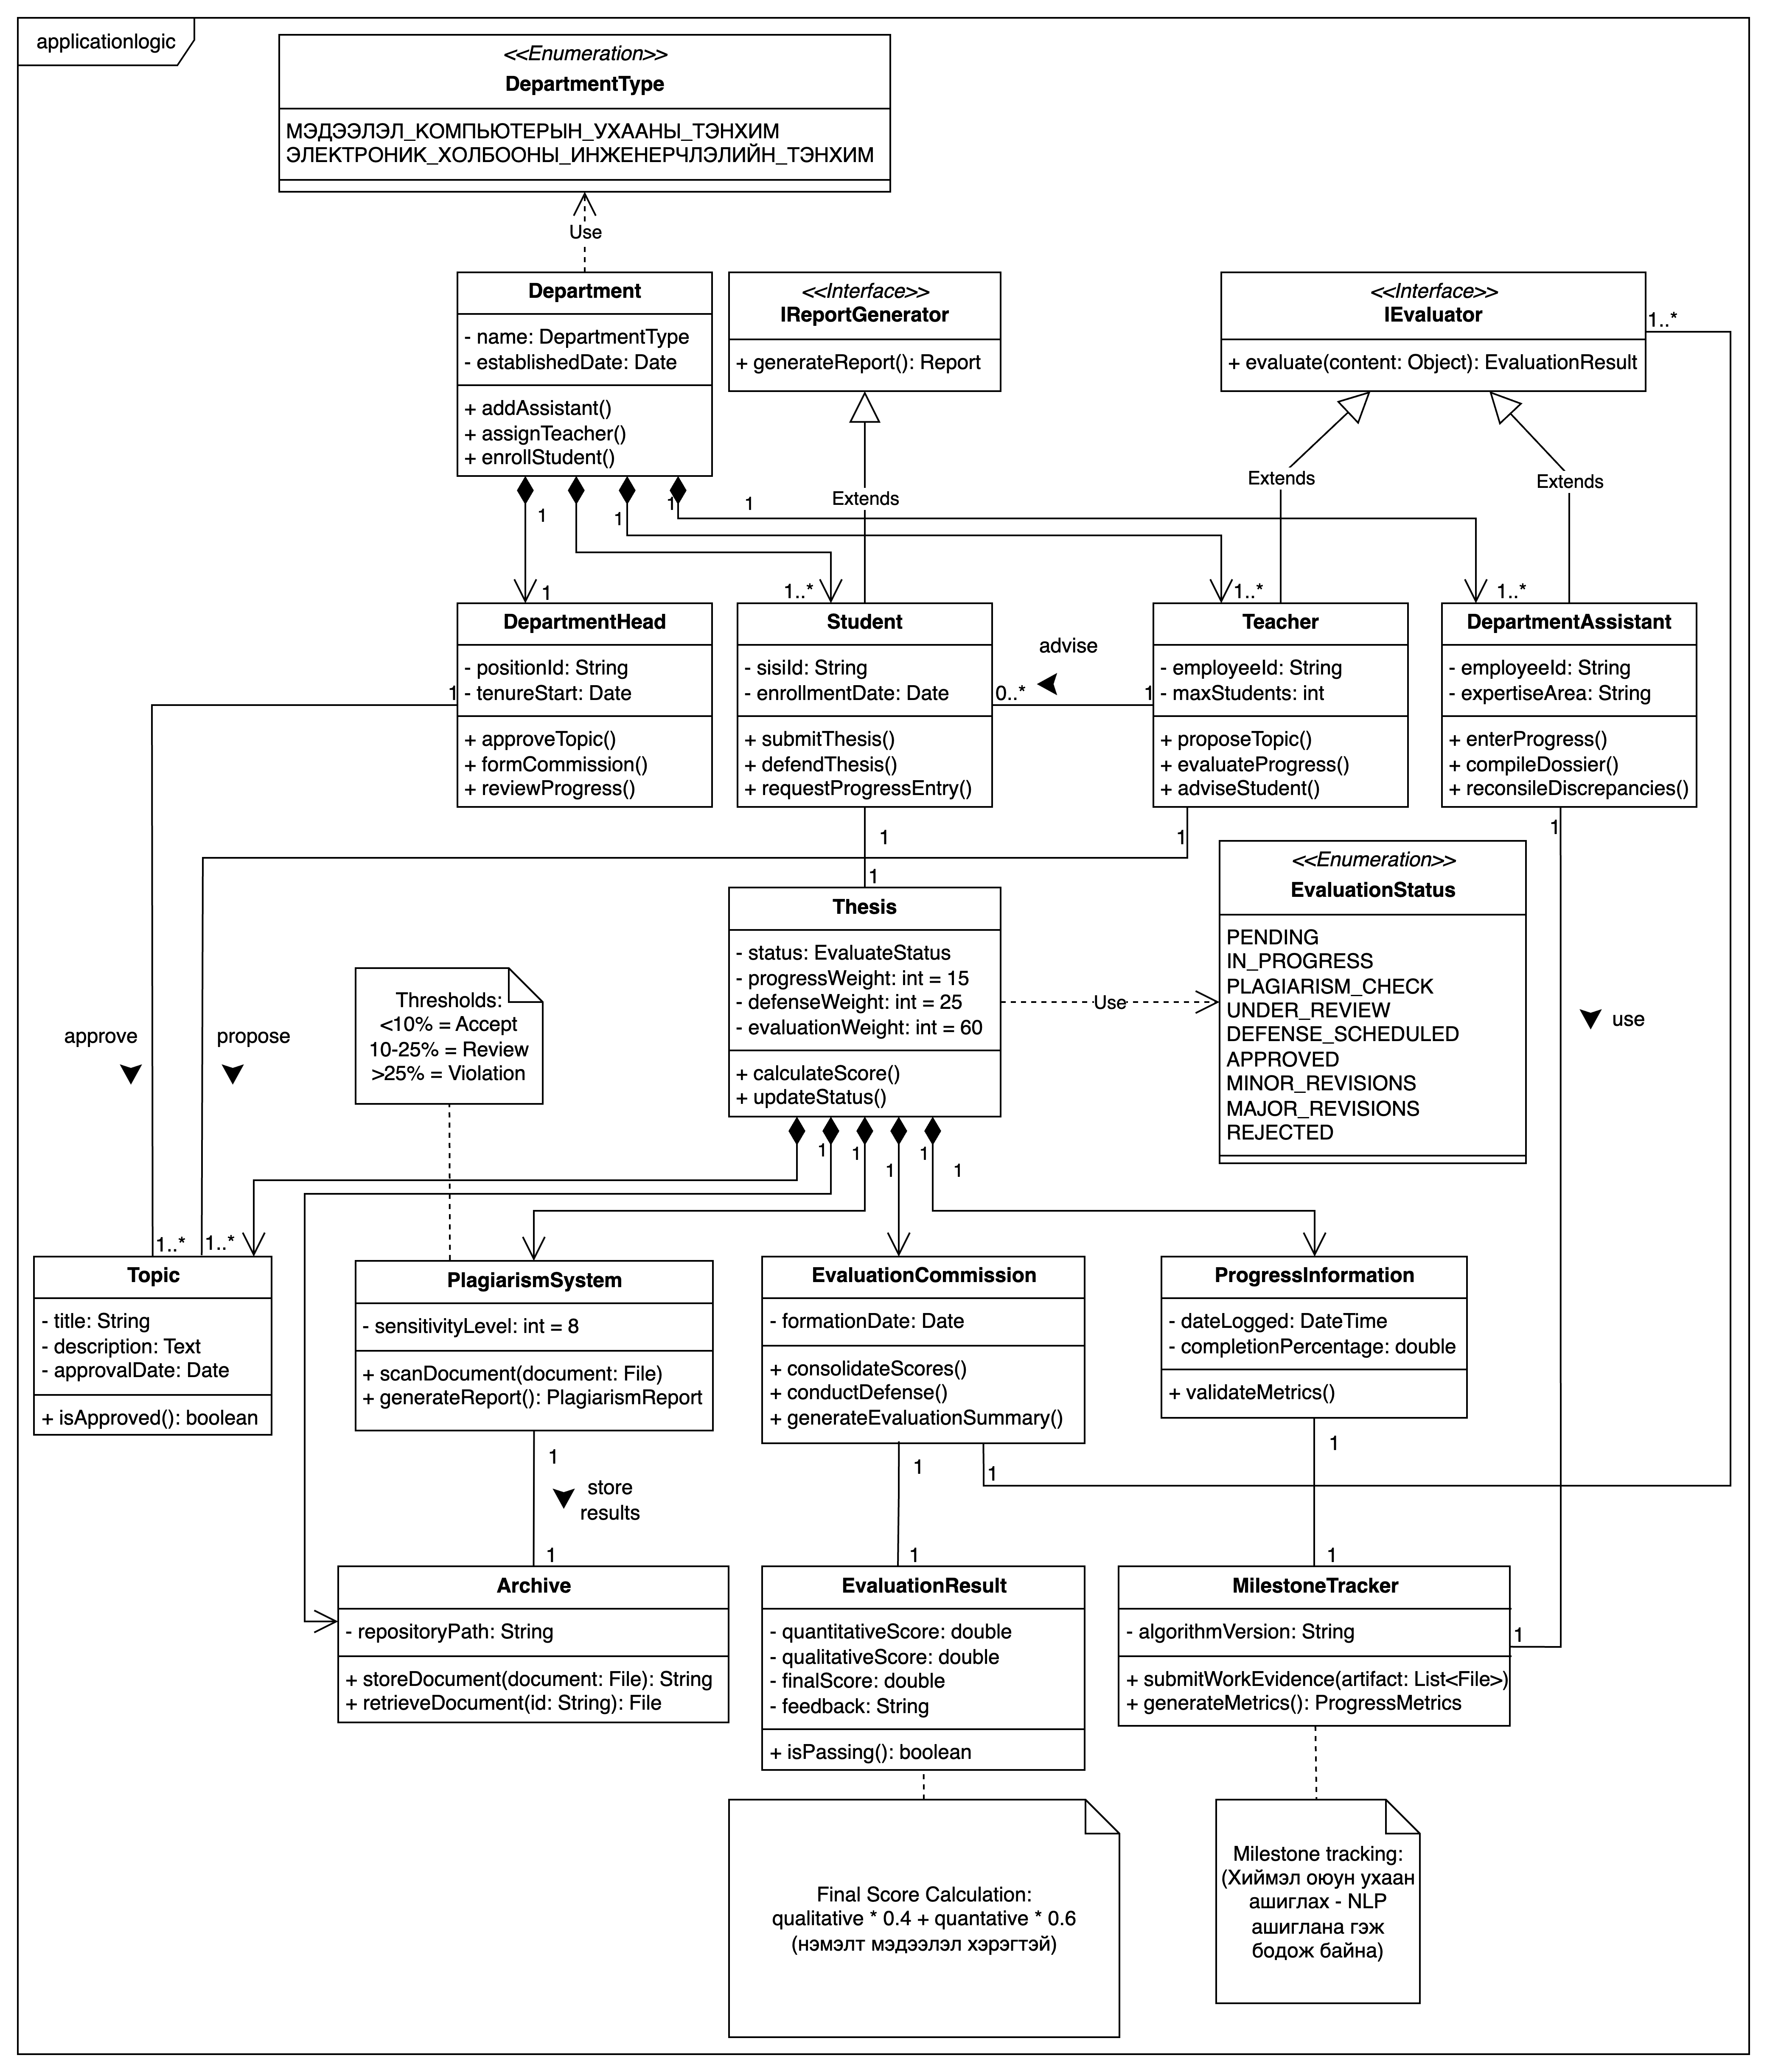
\includegraphics[width=17cm]{images/image.png}
	\caption{Дипломын ажлыг удирдах системийн классын диаграм}
	\label{fig:image}
\end{figure}